% \begin{figure}
% %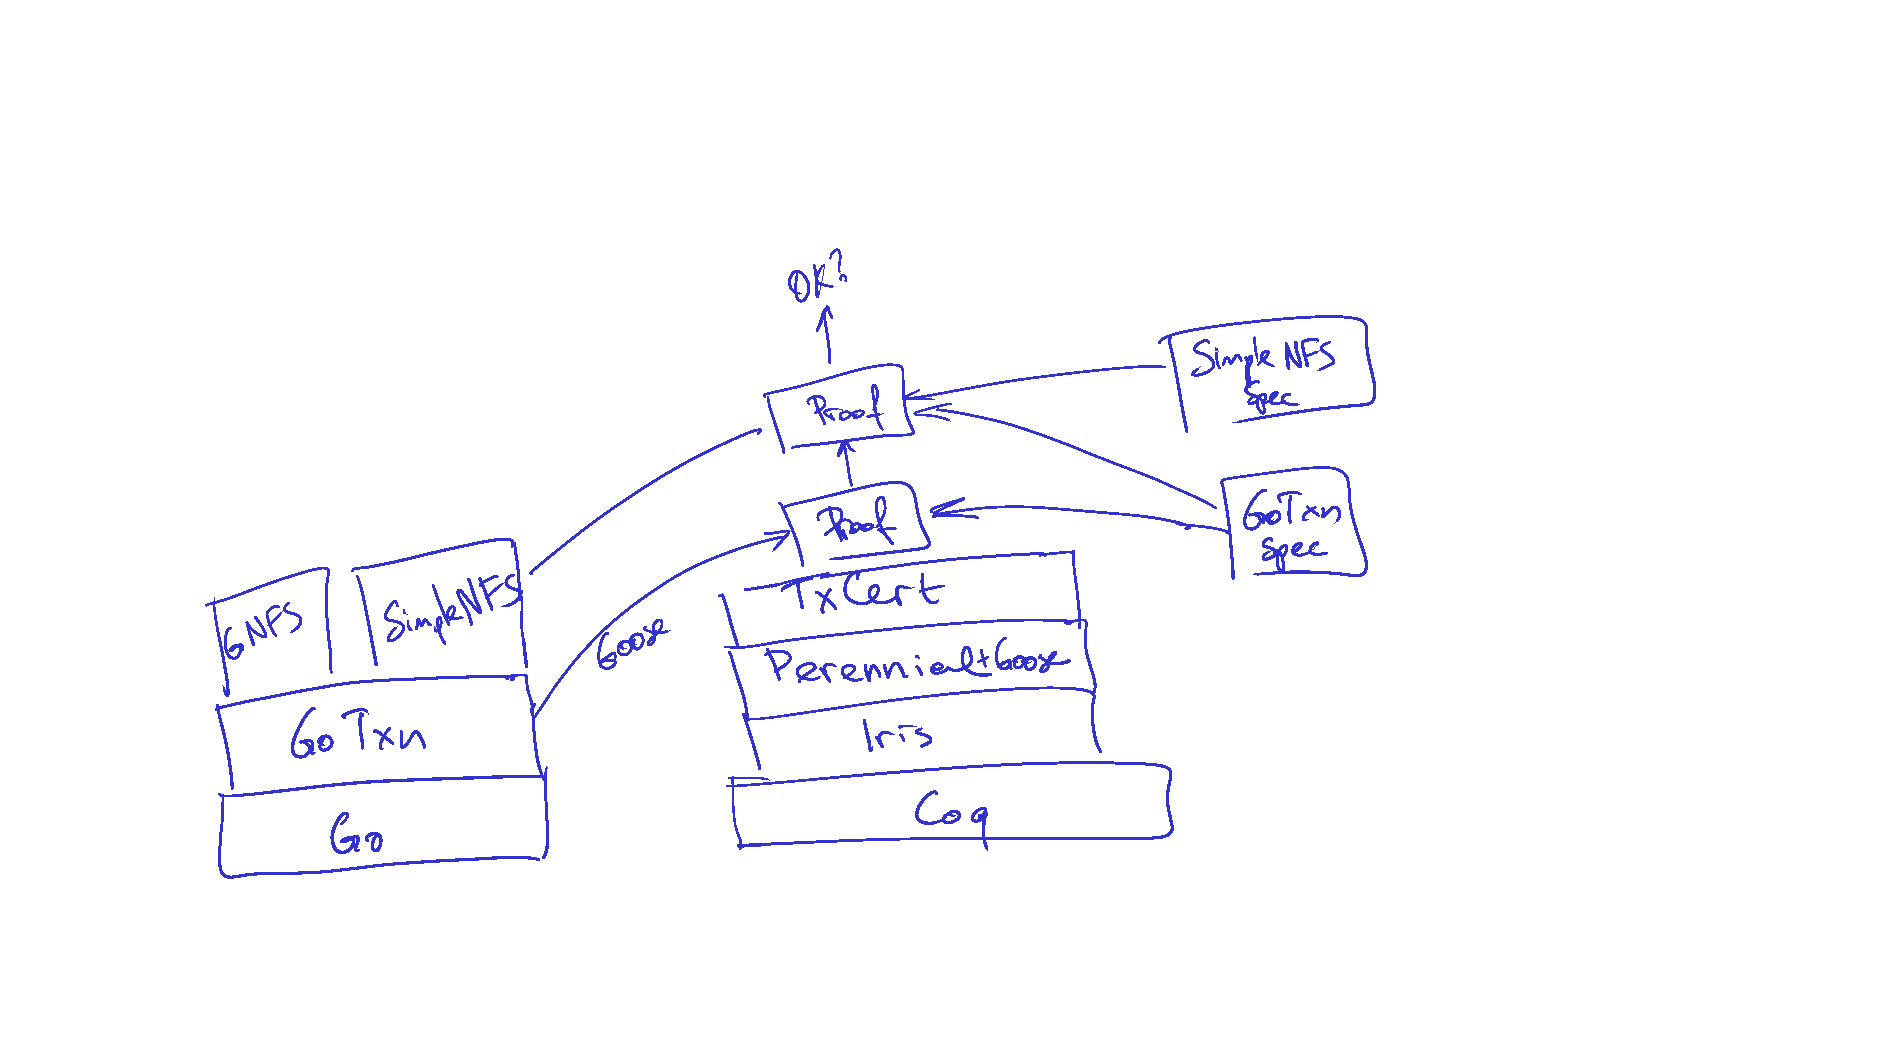
\includegraphics[width=\columnwidth]{fig/overview}
% \includegraphics{drawn-diagrams/jrnl-overview.png}
% \caption{Overview of Perennial, \txn, \simplenfs, and \gnfs.}
% \label{fig:overview}
% \end{figure}

\begin{figure}
\begin{tikzpicture}[>=latex, node distance=.5cm]

  \tikzstyle{other}=[fill=gray!20];

  \tikzstyle{layer}=[thick,rectangle, draw,minimum width=3.65cm,minimum
    height=.5cm, align=center];
  \tikzstyle{layerthin}=[outer sep=0, thick,rectangle, draw,minimum width=3.65cm,minimum
    height=.5cm, align=center];

  \tikzstyle{layermini}=[thick,rectangle, draw, minimum width=1.5cm,minimum height=.5cm,align=center];
  \tikzstyle{layerhalf}=[thick,rectangle, draw, minimum width=1.95cm,minimum height=.5cm,align=center];
  \tikzstyle{layeroverhalf}=[thick,rectangle, draw, minimum width=2.25cm,minimum height=.5cm,align=center];

  \tikzstyle{layers}=[thick,rectangle, draw, minimum
    width=1.75cm,minimum height=1cm,align=center];

  \tikzstyle{edge}=[->,thick];
  
  \draw node (coq) [layerthin, other] {Iris + Coq};
  %\draw node (iris) [layer, other,above of=coq] {Iris};
  %\draw node (goose) [layer, other, above of=iris] {Perennial + Goose};
  \draw node (jrnlcert) [layerthin, above of=coq] {Perennial 2.0};

  \draw node (go) [layerthin, other, left=1cm of jrnlcert] {Go};
  \draw node (gojrnl) [layer, above of=go] {\txn};
  \draw node (gnfs) [layermini, above=of gojrnl.west,anchor=west] {\gnfs};
  \draw node (simplenfs) [layerhalf, above=of gojrnl.east,anchor=east] {\simplenfs};
  \draw node (recexamp) [layerhalf, above of=simplenfs, font=\footnotesize] {Toy Client};

  \draw node (gojrnlspec) [layeroverhalf, above=.75cm of jrnlcert.east,anchor=east, font=\footnotesize] {\txn Spec};
  \draw node (simplenfsspec) [layeroverhalf, above of=gojrnlspec, font=\footnotesize] {\simplenfs Spec};
  \draw node (recspec) [layeroverhalf, above of=simplenfsspec, font=\footnotesize] {Example Spec};


  \tikzstyle{proofnode}=[dashed,rectangle, draw, minimum width=1.25cm,minimum height=.5cm,align=center];
  \draw node (proof1) [proofnode, above=0cm of jrnlcert.north west,anchor=south west] {Proof};
  \draw node (proof2) [proofnode, above of=proof1] {Proof};
  \draw node (proof3) [proofnode, above of=proof2] {Proof};

  \draw node (bin) [above=2.15cm of gojrnl] {\cc{a.out}};
  \draw [edge] (gojrnl.north)+(0,1.25cm) -- node[left] {\cc{go build}} (bin.south);

  \draw [edge, shorten >=.15cm, shorten <=.15cm] (gojrnl) -- (proof1);
  \draw [edge, shorten >=.15cm, shorten <=.15cm] (simplenfs) -- (proof2);
  \draw [edge, shorten >=.15cm, shorten <=.15cm] (recexamp) -- node[above] {Goose} (proof3);

  \path let \p1=(bin) in let \p2=(proof3) in node (ok) at (\x2, \y1) {OK?};
  \draw [edge, transform canvas={xshift=3.45cm}] (gojrnl.north)+(0,1.25cm) -- (bin.south);
  %\draw [edge, shorten >=.15cm, shorten <=.15cm] (proof3) -- node[right] {{\tt coqc}} (ok);

  %{\cc{go build}};
  % \draw node (coqgo) [layerm,above=of goose,anchor=north] {Coq
  %   representation of Go (\cref{ch:goose})};
  % \draw node (perennial) [layerm,above=of iris.east,anchor=east] {\sys library
  %   for\\concurrency and recovery (\cref{ch:proving})};
  % \draw node (proof) [layers,above=of perennial.west,anchor=west,fill=green!10,dashed] {Proof};
  % \draw node (spec) [layers,above= of perennial.east,anchor=east,fill=green!10,dashed] {Spec};

  % \draw node (code) [layers,left of=coqgo,node distance=5cm,fill=green!10,dashed] {Go src};
  % \draw node (bin) [layers,below=of code] {a.out};
  % \draw [edge] (code.south) -- node[right] {Go compiler} (bin.north);

  % \draw [edge] (code.east) -- node[above] {Goose} node[below] {Translator} (coqgo.west);
  % \draw [edge] (coqgo.east) -- (proof.west);
  % \draw [edge] (spec.west) -- (proof.east);

  % \draw [edge] (proof.north) -- node[above] {OK?} ($(proof.north)+(0.0,+0.3)$);
          
\end{tikzpicture}

\caption{Overview of Perennial, \txn, \simplenfs, and \gnfs.}
\label{fig:overview}
\end{figure}

\cref{fig:overview} gives an overview of how \txn and systems
building on it are verified using Perennial.
On the left of the figure is the executable code, which is written
in Go. On top of \txn, we have implemented two NFS servers to evaluate \txn
along different dimensions. \gnfs is a functional NFS server that is sufficient
to run real applications, which we use to assess \txn's scalability and
performance. Meanwhile, \simplenfs is a verified, core subset of \gnfs's
functionality, which evaluates the usability of \txn's specs for building
verified systems on top of it.
% \gnfs supports most of RFC 1813~\cite{RFC:1813}, with
% the exception of symbolic links and permissions.  \gnfs supports the
% \cc{unstable} argument to the write RPC, allowing for writes that are
% not immediately flushed to disk, as well as the commit RPC that flushes
% these writes.  To allow this, \txn supports transactions that commit
% but are not immediately flushed to disk.  To formally validate the
% specifications of \txn, we verified \simplenfs, a core subset of \gnfs.

On the right side of the figure is the verification stack. The verification
builds on the Perennial 2.0 framework, which is itself implemented in the Iris
framework in the Coq proof assistant. To reason about executable code, a tool
called Goose translates a Go implementation into a model that we can prove
specifications about in Perennial. Perennial provides a model of execution for
Go code that incorporates crash-safety and concurrency, which
includes a model of the disk (with atomic, synchronous reads and writes of 4KB
sectors) as well as a model of crashes and recovery (crashes at arbitrary points
during execution, and jumping to specific boot code for recovery after a crash).

\txn's top-level specification describes its API in terms of an extension of
concurrent separation logic, with pre-, post-, and crash conditions. These
specifications capture the behavior of individual Go functions: if the function
is run in a state satisfying its precondition, then the final state will satisfy
the postcondition, and if the system crashes the state will satisfy the crash
condition. The specification for the journaling API is described in detail in \cref{s:design}. We
demonstrate the usefulness of this specification by proving correctness of the \simplenfs
server using logically atomic crash specifications (\cref{s:proof:logatom}). %, a style of specification
%encoded in Hoare triples.
The top-level theorem for \simplenfs states that its RPCs
atomically follow transitions of a state machine formalizing the NFSv3 protocol (based on RFC
1813~\cite{RFC:1813}).

As described in FSCQ and Argosy~\cite{chen:fscq,chajed:argosy}, crash conditions
can be used to reason about recovery procedures, even crashes during recovery. A
recovery procedure can safely be re-run after a crash if its specification is
\emph{idempotent}: its crash condition should imply its precondition. As an
end-to-end check of the crash specs in \simplenfs and \txn, showing they support
recovery correctly, we prove an idempotent specification for a toy example
client on top of \simplenfs, establishing that it can successfully execute even if
\simplenfs crashes and recovers an arbitrary number of times.

The proof of \txn's specification depends on a number of assumptions. We assume
that the disk writes 4KB blocks atomically, even on crash, and assume that the
code executes according to the Perennial model generated by Goose. The
specification relies on the caller to provide concurrency control; the proof of
\simplenfs checks that locking is performed correctly, but \gnfs is unverified
and we trust that its concurrency control is correct in order to make operations
atomic (though this does not say they correctly implement the NFS
specification).

% \begin{figure}[ht]
%   \begin{Verbatim}[commandchars=\\\{\},codes={\catcode`\$=3\catcode`\^=7\catcode`\_=8},fontsize=\small]
\PY{c}{(*}\PY{c}{ The state of SimpleNFS is a map from file handles}
\PY{c}{(}\PY{c}{inode numbers}\PY{c}{)}\PY{c}{ to contents }\PY{c}{(}\PY{c}{list of bytes}\PY{c}{)}\PY{c}{. }\PY{c}{*)}
\PY{k+kn}{Definition} \PY{n}{State} \PY{o}{:=} \PY{n}{gmap} \PY{n}{fh} \PY{o}{(}\PY{n}{list} \PY{n}{u8}\PY{o}{)}\PY{o}{.}

\PY{k+kn}{Definition} \PY{n}{write} \PY{o}{(}\PY{n}{f} \PY{o}{:} \PY{n}{fh}\PY{o}{)} \PY{o}{(}\PY{n}{off} \PY{o}{:} \PY{n}{u64}\PY{o}{)}
           \PY{o}{(}\PY{n}{d} \PY{o}{:} \PY{n}{list} \PY{n}{u8}\PY{o}{)} \PY{o}{(}\PY{n}{d0} \PY{o}{:} \PY{n}{list} \PY{n}{u8}\PY{o}{)}
    \PY{o}{:} \PY{n}{transition} \PY{n}{State} \PY{n}{u32} \PY{o}{:=}
  \PY{c}{(*}\PY{c}{ Convert u64 to mathematical integer }\PY{c}{*)}
  \PY{k}{let} \PY{n}{off} \PY{o}{:=} \PY{n}{int}\PY{o}{.}\PY{n}{nat} \PY{n}{off} \PY{k}{in}
  \PY{c}{(*}\PY{c}{ Simplified spec does not allow creating holes,}
\PY{c}{     but does allow appending }\PY{c}{*)}
  \PY{n}{check} \PY{o}{(}\PY{n}{off} ≤ \PY{n}{length} \PY{n}{d0}\PY{o}{)}\PY{o}{;}
  \PY{k}{let} \PY{n}{d\PYZsq{}} \PY{o}{:=} \PY{n}{d0}\PY{o}{[}\PY{o}{:}\PY{n}{off}\PY{o}{]} \PY{o}{+}\PY{o}{+} \PY{n}{d} \PY{o}{+}\PY{o}{+} \PY{n}{d0}\PY{o}{[}\PY{n}{off}\PY{o}{+}\PY{n}{length} \PY{n}{d}\PY{o}{:}\PY{o}{]} \PY{k}{in}
  \PY{c}{(*}\PY{c}{ Update spec file state }\PY{c}{*)}
  \PY{n}{modify} \PY{o}{(}\PY{k}{fun} \PY{n}{s} \PY{o}{=\PYZgt{}} \PY{n}{insert} \PY{n}{f} \PY{n}{d\PYZsq{}} \PY{n}{s}\PY{o}{)}\PY{o}{;}
  \PY{n}{ret} \PY{o}{(}\PY{n}{U32} \PY{o}{(}\PY{n}{length} \PY{n}{d}\PY{o}{)}\PY{o}{)}\PY{o}{.}
\end{Verbatim}

%   \vspace{-\baselineskip}
%   \caption{Specification for an NFS \textsc{write} which writes \cc{d} to
% file handle \cc{f} at offset \cc{off}. A wrapper around the spec checks that
% \cc{f} is a valid handle, passes the current file contents \cc{d0}, and allows
% the spec to return an error (e.g., if out of disk space). }
%   \label{fig:nfswritespec}
% \end{figure}
%
% \joe{We should probably trim this down now, since we don't much care about SimpleNFS's TCB anymore. Maybe rephrase it in terms of GoJournal's tcb?}
% The end-to-end proof for an application using \txn, such as \simplenfs, depends on a number of assumptions.
% The proof itself relies on the Coq proof assistant being correct, and
% on the top-level specification of \simplenfs correctly capturing its
% intended behavior.  The proof also relies on Goose to faithfully model
% the Go code of \simplenfs and \txn in Coq, and on the Go compiler and
% runtime to correctly execute the code.  The proof also assumes that the
% disk model is accurate (atomic and synchronous sector writes).  Finally,
% the proof does not cover the code that parses XDR-encoded RPC requests.
% We use a separate tool to generate this Go code from an XDR description
% of the protocols~\cite{RFC:1813, RFC:1057, RFC:4506}.
